% BSD 3-Clause License
%
% Copyright (c) 2023 Quux System and Technology. All rights reserved.
%
% Redistribution and use in source and binary forms, with or without
% modification, are permitted provided that the following conditions are met:
%
% 1. Redistributions of source code must retain the above copyright notice, this
%    list of conditions and the following disclaimer.
%
% 2. Redistributions in binary form must reproduce the above copyright notice,
%    this list of conditions and the following disclaimer in the documentation
%    and/or other materials provided with the distribution.
%
% 3. Neither the name of the copyright holder nor the names of its
%    contributors may be used to endorse or promote products derived from
%    this software without specific prior written permission.
%
% THIS SOFTWARE IS PROVIDED BY THE COPYRIGHT HOLDERS AND CONTRIBUTORS "AS IS"
% AND ANY EXPRESS OR IMPLIED WARRANTIES, INCLUDING, BUT NOT LIMITED TO, THE
% IMPLIED WARRANTIES OF MERCHANTABILITY AND FITNESS FOR A PARTICULAR PURPOSE ARE
% DISCLAIMED. IN NO EVENT SHALL THE COPYRIGHT HOLDER OR CONTRIBUTORS BE LIABLE
% FOR ANY DIRECT, INDIRECT, INCIDENTAL, SPECIAL, EXEMPLARY, OR CONSEQUENTIAL
% DAMAGES (INCLUDING, BUT NOT LIMITED TO, PROCUREMENT OF SUBSTITUTE GOODS OR
% SERVICES; LOSS OF USE, DATA, OR PROFITS; OR BUSINESS INTERRUPTION) HOWEVER
% CAUSED AND ON ANY THEORY OF LIABILITY, WHETHER IN CONTRACT, STRICT LIABILITY,
% OR TORT (INCLUDING NEGLIGENCE OR OTHERWISE) ARISING IN ANY WAY OUT OF THE USE
% OF THIS SOFTWARE, EVEN IF ADVISED OF THE POSSIBILITY OF SUCH DAMAGE.
%
\begin{recipe}{松子肉}

\ingredients

\ingredient{豆油皮}{一张}
\ingredient{萝卜}{四两五}
\ingredient{猪肉}{二两}
\ingredient{鸡蛋}{二个}
\ingredient{胡椒}{三分}
\ingredient{菜油}{一斤耗一两五}
\ingredient{干豆粉}{三钱}
\ingredient{奶汤}{四两}
\ingredient{二汤}{二两}
\ingredient{盐}{五分}
\ingredient{味精}{二分}
\ingredient{松子}{二钱}
\ingredient{葱}{二钱}
\ingredient{姜}{六分}

\preparation

\step 选用肥瘦相连的猪肉,洗净,切成二寸长、一分半厚的细丝。松子去皮捶茸放于肉
丝中。萝卜去皮,切成二分厚、二寸长的粗丝,挤干水。姜、葱均切成细丝。

\step 鸡蛋去壳与干豆粉调匀成为蛋清豆粉,加入味精、盐、
\begin{wrapfigure}[7]{l}{17em}%
\centering%
\vspace{-.4375\baselineskip}%
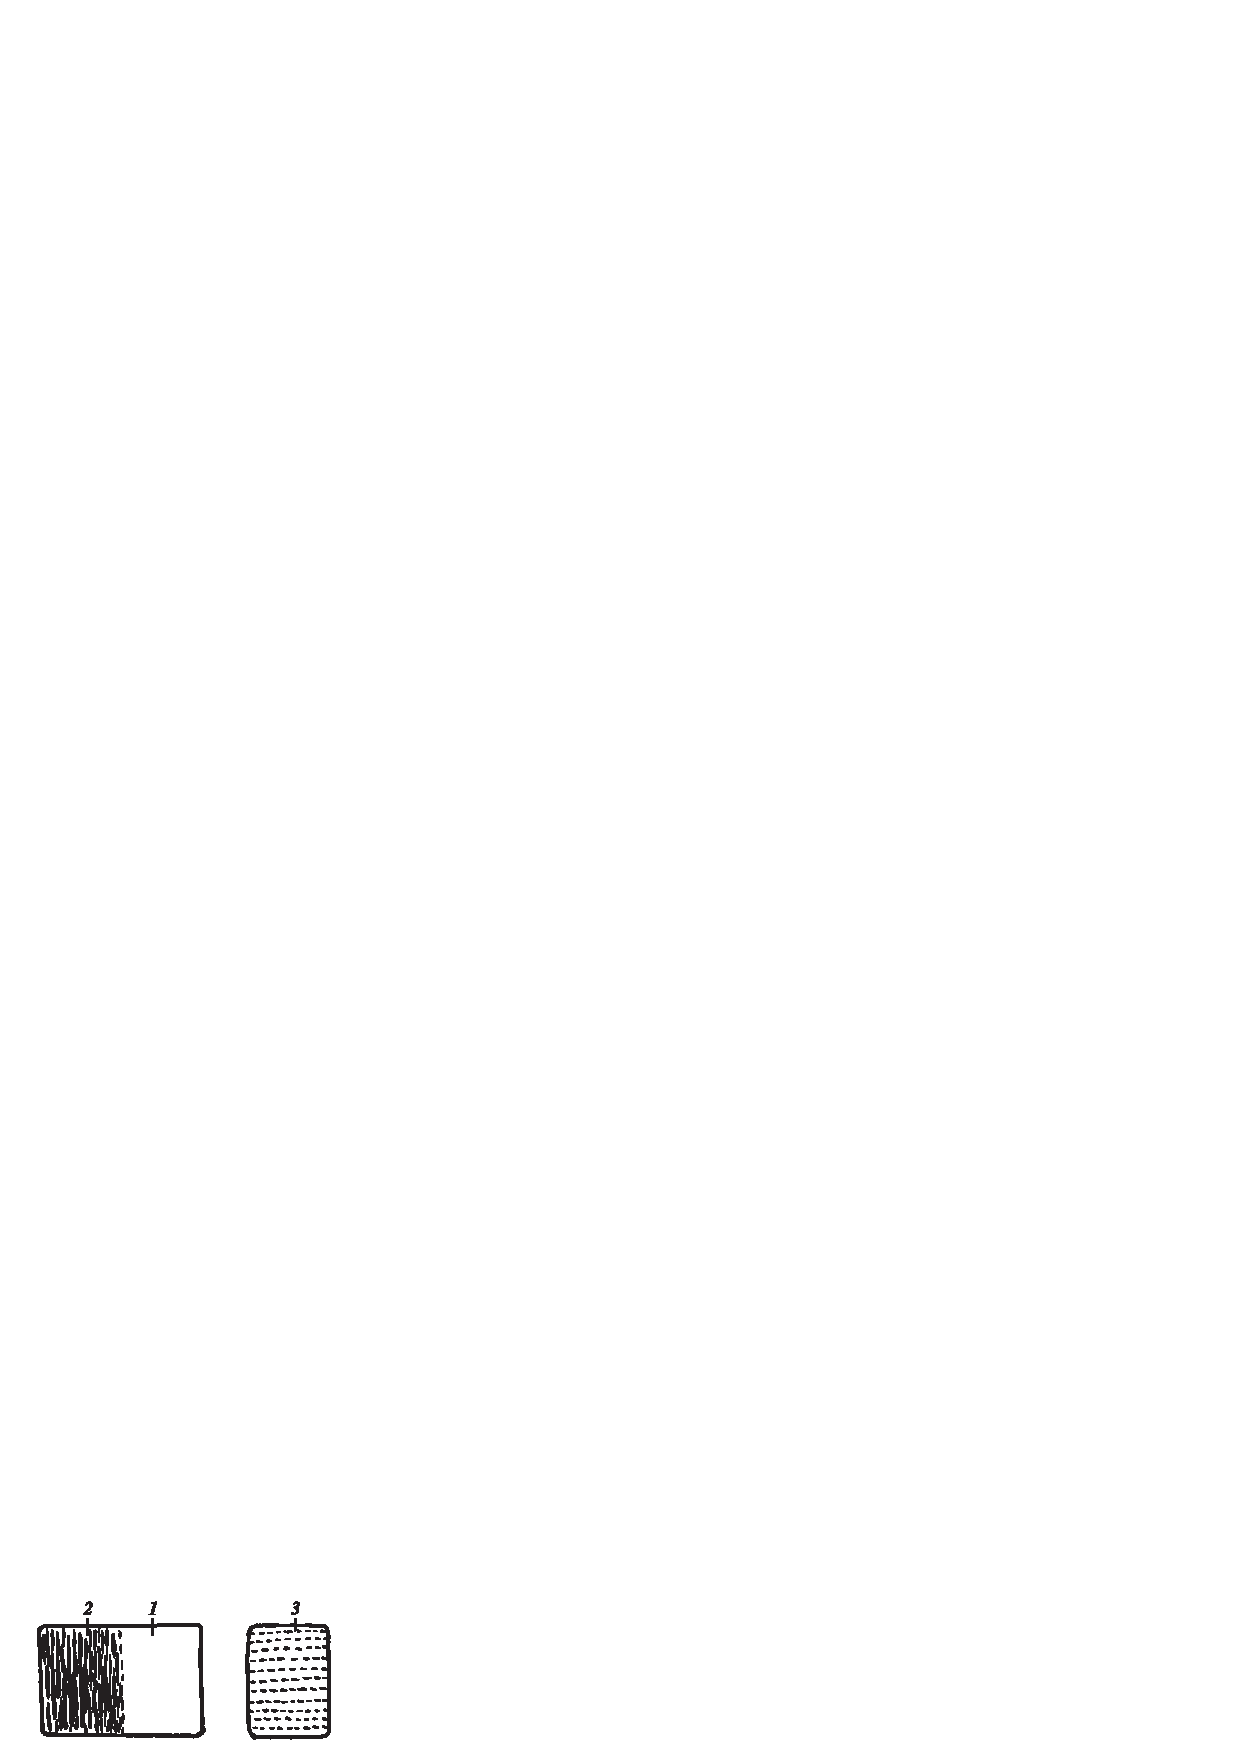
\includegraphics[scale=1]{illustration-003.pdf}%
\vspace{-.5625\baselineskip}%
\caption{松子肉包叠法图}%
\label{松子肉包叠法图}%
{\small 1.豆油皮\hspace{1em}2.肉丝\hspace{1em}3.叠好后}%
\end{wrapfigure}%
胡椒,于深碗中混合好,再与猪肉丝、萝卜丝、姜、葱一并拌匀。

\step 豆油皮一张修成六寸宽、八寸长,平铺案板上,而后把拌匀的猪肉丝、萝卜丝等铺
在豆油皮上,铺成七分厚,铺上豆油皮的一半,再把另一半叠过来,接头处涂蛋清豆粉封
口,如图\,\ref{松子肉包叠法图}\,。

\step 炒锅倒入菜油烧红,将叠好的豆油皮包放入炸透,炸成金黄色,泌去炸油,放盘中
晾冷。再用刀切成一寸半长、
\begin{wrapfigure}[5]{l}{10em}%
\centering%
\vspace{-1.25\baselineskip}%
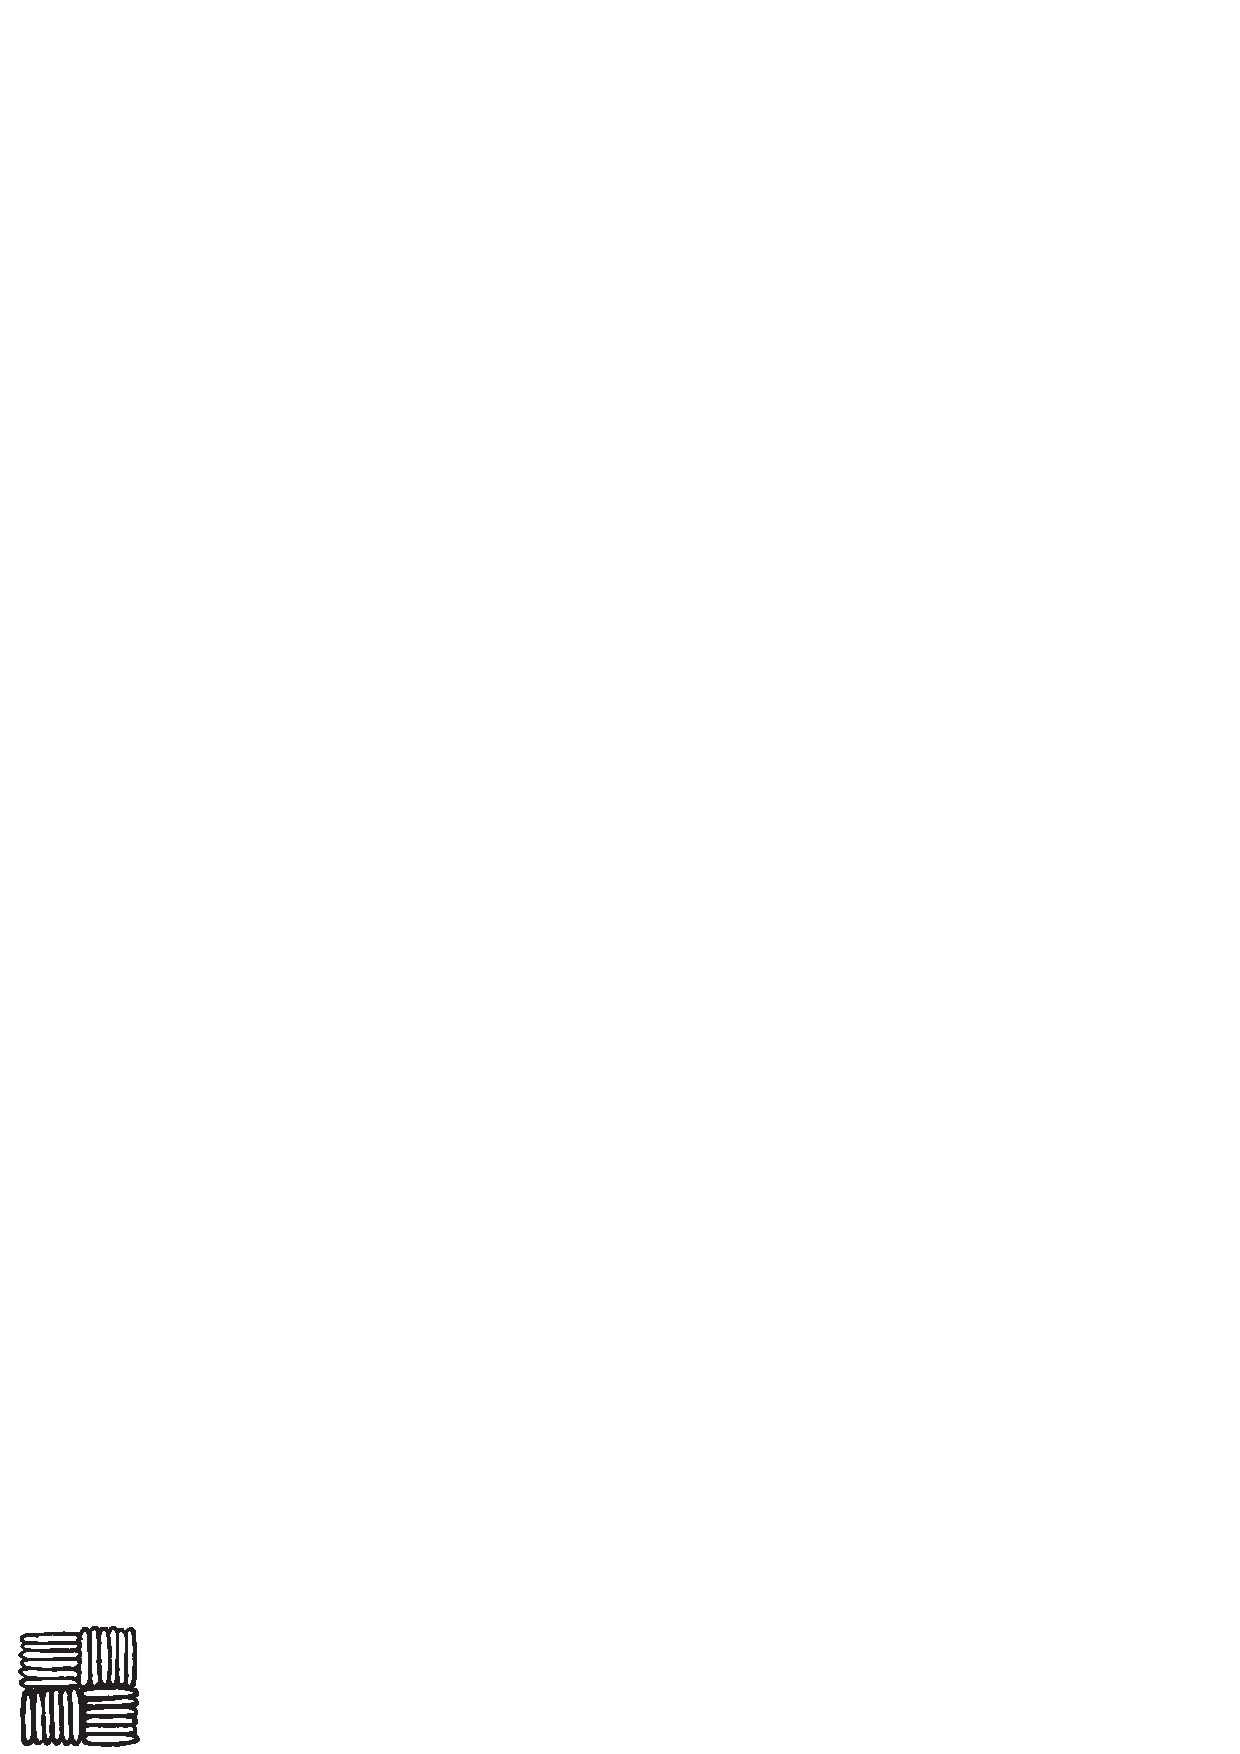
\includegraphics[scale=1]{illustration-004.pdf}%
\vspace{-.5625\baselineskip}%
\caption{松子肉摆法}%
\label{松子肉摆法}%
\end{wrapfigure}%
三分宽、七分厚的长条,共二十四条。以六条为一组,于碗中镶成卍字形,如
图\,\ref{松子肉摆法}\,。然后加二汤淹没肉条,上笼蒸三十分钟取出,扣于碗内,再加
奶汤四两、盐七分即成。

\features

此菜香软可口,营养丰富,特别适于冬季食用。

\end{recipe}

% vim: filetype=tex noautoindent nojoinspaces
% vim: fileencoding=utf-8 formatoptions+=m
% vim: textwidth=78 tabstop=4 shiftwidth=4 softtabstop=4
